\documentclass[a4paper,11pt]{article}
\usepackage{fullpage}
\usepackage{standalone}
\usepackage[utf8]{inputenc}
\usepackage[british]{babel}
\usepackage{csquotes}
\usepackage[T1]{fontenc}
\usepackage{amsmath}
\usepackage{amssymb}
\usepackage{mathtools}
\usepackage{mathptmx}
\usepackage{natbib}
\usepackage[final,babel]{microtype}
\usepackage[colorlinks,linkcolor=blue,citecolor=blue,urlcolor=blue]{hyperref}
\usepackage{doi}
\usepackage{siunitx}
\usepackage[margin=3pt]{subcaption}
\usepackage{xcolor}
\PassOptionsToPackage{final}{graphicx}
\usepackage{tikz}
\usetikzlibrary{arrows}
\usetikzlibrary{patterns}
\usepackage{bm}
\usepackage{booktabs}
\usepackage{tabularx}
\usepackage{enumitem}
\usepackage{titlesec}

\title{
\vspace*{-2em}
Monitoring Committee Progress Report \#4\\
\vspace*{1em}
\Large{Numerical Representation of Mountains in Atmospheric Models}}
\author{James Shaw
\vspace{0.5em} \\
\large{Supervisors: Hilary Weller, John Methven, Terry Davies}
\vspace{0.5em} \\
\large{Monitoring Committee: Paul Williams, Maarten Ambaum}}
\date{24th November 2016}

\captionsetup{margin=3pt,font={small}}
%\setlength{\bibsep}{0.3em plus 0.1ex}

\makeatletter
\AtBeginDocument{
  \hypersetup{
    pdftitle = {Monitoring Committee Progress Report \#4},
    pdfauthor = {James Shaw}
  }
}
\makeatother

\makeatletter
\patchcmd{\ttlh@hang}{\parindent\z@}{\parindent\z@\leavevmode}{}{}
\patchcmd{\ttlh@hang}{\noindent}{}{}{}
\makeatother

\newcommand{\TODO}[1]{\textcolor{purple}{TODO: \emph{#1}}}
\newcommand{\iu}{{i\mkern1mu}}

\defcitealias{openfoam}{{OpenFOAM user guide}}
\begin{document}
\maketitle

\section{Introduction}

An atmospheric model solves the equations of motion in discrete form on a numerical mesh.  This mesh becomes distorted over sloping terrain, and the distortions can lead to larger numerical errors.  With new atmospheric models using increasingly fine mesh spacing, steep slopes become resolved by the mesh.  These steep slopes can result in highly-distorted meshes that can lead to larger numerical errors.  My PhD project seeks out new techniques for reducing numerical errors in regions of steep terrain.

There are several methods for representing terrain on a mesh.  Operational models use some form of terrain-following transformation that distorts horizontal mesh layers to accommodate the terrain.  Such meshes are straightforward to represent using a uniform rectangular computational mesh, but sloped terrain distorts the mesh far above the surface, leading to larger errors \citep{schaer2002,klemp2011}.  The cut cell method is an alternative to terrain-following transformations in which a piecewise linear representation of the surface is intersected with a uniform rectangular mesh.  Cut cell meshes are less distorted than terrain-following meshes, but the cut cell method creates arbitrarily small cells that impose severe timestep constraints on explicit numerical methods \citep{klein2009}.  Other representations of terrain have also been used, such as the sloping step method used in the Eta model \citep{mesinger2012} and unstructured tetrahedral meshes \citep{smolarkiewicz-szmelter2011}.

The wide variety of mesh types motivates the development of finite volume methods for arbitrary meshes.  This enables a like-for-like comparison between different types of mesh and allows us to assess the characteristics of new types of mesh.  Further, we hope that the new methods we develop will be less sensitive to mesh distortions compared to traditional methods.

My project comprises three parts.  First, a new type of mesh called the slanted cell mesh has been developed that is less distorted than terrain-following meshes and avoids arbitrarily small cells that are associated with the cut cell method \citep{shaw-weller2016}.  Second, we have designed an explicit, Eulerian transport scheme that is accurate near highly-distorted lower boundaries and is suitable for a variety of mesh types.  Third, we intend to generalise the Charney--Phillips staggering for arbitrary meshes and hope that this new formulation will alleviate the computational mode that is associated with the Lorenz staggering of variables \citep{arakawa-konor1996}.

\section{A new finite volume scheme for transport over steep slopes}
In May 2016, monitoring committee report \#3 (hereafter MC3) described our progress developing an explicit, Eulerian transport scheme which has been named ``cubicFit''.  At that time the scheme was numerically unstable on some meshes.  We have since improved stability using additional constraints derived from a von Neumann analysis.  No further stability problems have been encountered since the improvement was implemented.  In this section, an overview of the cubicFit scheme is provided, and some details of the von Neumann stability analysis are outlined.

The discretisation starts from the flux form transport equation of a dependent variable $\phi$,
\begin{align}
	\frac{\partial \phi}{\partial t} - \nabla \cdot \left( \mathbf{u} \phi \right) = 0 \label{eqn:transport}
\end{align}
where $\mathbf{u}$ is the wind field.  A C-grid staggering is used such that the dependent variable $\phi$ is prognosed at cell centroids and the wind is prescribed at face centroids.  The divergence term in equation~\eqref{eqn:transport} is discretised using Gauss' divergence theorem,
\begin{align}
	\nabla \cdot \left( \mathbf{u} \phi \right) \approx \sum_{f \in\:c} \mathbf{u}_f \cdot \mathbf{S}_f \phi_F
\end{align}
where $\sum_{f \in\:c}$ denotes a summation over faces $f$ of cell $c$, $\mathbf{u}_f$ is the wind vector prescribed at the face, and $\mathbf{S}_f$ is the vector that is outward normal to the face having a magnitude equal to the face area.  $\phi_F$ is an approximation of the dependent variable at the face centroid.  The accuracy of this approximation is crucial to the accuracy of the transport scheme.

\begin{figure}
	\centering
	\subcaptionbox{12-point stencil for a face in the interior of a two-dimensional quadrilateral mesh \label{fig:stencil-interior}}[.32\linewidth]{\TODO{}}
	\subcaptionbox{6-point stencil for a face near a flat lower boundary \label{fig:stencil-boundary}}[.32\linewidth]{\TODO{}}
	\subcaptionbox{9-point stencil for a face near a sloping lower boundary.  When the slope is only slight then there is insufficient variation in $x$ to fit the $x^3$ polynomial term. \label{fig:stencil-sloped}}[.32\linewidth]{\TODO{}}
	\caption{Example stencils for different regions of quadrilateral meshes.  The wind direction $\mathbf{u}$ and local $x$--$y$ coordinate system is indicated for each stencil.  The values of the dependent variable $\phi$ immediately upwind and downwind of face $f$ are labelled $\phi_u$ and $\phi_d$ respectively.}
	\label{fig:stencils}
\end{figure}

The cubicFit scheme approximates the value $\phi_F$ by fitting a multidimensional polynomial over a stencil of cell centre values using a least-squares approach.  An example stencil for a face in the interior of a two-dimensional quadrilateral mesh is shown in figure~\ref{fig:stencil-interior}.  The cell centre values immediately upwind and downwind of face $f$ are labelled $\phi_u$ and $\phi_d$ respectively.
The polynomial for such a face is
\begin{align}
	\phi = a_1 + a_2 x + a_3 y + a_4 x^2 + a_5 xy + a_6 y^2 + a_7 x^3 + a_8 x^2 y + a_9 x y^2 \label{eqn:nine-poly}
\end{align}
By choosing a local coordinate with its origin positioned at the face centroid then $\phi_F = a_1$.  The value of $\phi_F$ is calculated as a weighted sum of cell centre value,
\begin{align}
	\phi_F = \begin{bmatrix}w_u \\ w_d \\ w_3 \\ \vdots \\ w_n\end{bmatrix} \cdot
		\begin{bmatrix}\phi_u \\ \phi_d \\ \phi_3 \\ \vdots \\ \phi_n\end{bmatrix}
	= \mathbf{w} \cdot \bm{\phi}
\end{align}
where $n$ is the number of cells in the stencil for face $f$.  By convention the upwind cell is the first component and the downwind cell is the second component.

For stencils near boundaries (figure~\ref{fig:stencil-boundary}) and for stencils in some distorted mesh regions (figure~\ref{fig:stencil-sloped}), there is insufficient information to fit all nine polynomial terms in equation~\eqref{eqn:nine-poly}.  We can detect such cases by checking whether the matrix equation that results from the least squares procedure is numerically full rank (details are provided in MC3).

\begin{figure}
	\centering
	\subcaptionbox{2-point approximation \label{fig:vonNeumann-2}}[.25\linewidth]{\documentclass[tikz]{standalone}
\usepackage{bm}
\begin{document}
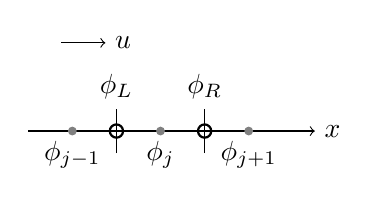
\begin{tikzpicture}[
  scale=0.56,
  cpnt/.style={fill=gray},
]

\draw [->] (-0.25,2) -- (0.75,2) node [right] {$u$};
\draw [->] (-1,0) -- (5.5,0) node [right] {$x$};
\draw (1,-0.5) -- (1,0.5) node [above] {$\phi_L$};
\draw (3,-0.5) -- (3,0.5) node [above] {$\phi_R$};

\path [cpnt] (0,0) circle [radius=0.1] node [below] {$\phi_{j-1}$};
\path [cpnt] (2,0) circle [radius=0.1] node [below] {$\phi_j$};
\path [cpnt] (4,0) circle [radius=0.1] node [below] {$\phi_{j+1}$};
\draw [thick] (1,0) circle [radius=0.15];
\draw [thick] (3,0) circle [radius=0.15];

\end{tikzpicture}
\end{document}
}
	\subcaptionbox{3-point approximation \label{fig:vonNeumann-3}}[.33\linewidth]{\documentclass[tikz]{standalone}
\usepackage{bm}
\begin{document}
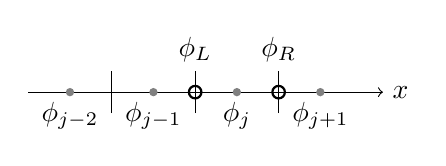
\begin{tikzpicture}[
  scale=0.53,
  cpnt/.style={fill=gray},
]

\draw [->] (-3,0) -- (5.5,0) node [right] {$x$};
\draw (-1,-0.5) -- (-1,0.5);
\draw (1,-0.5) -- (1,0.5) node [above] {$\phi_L$};
\draw (3,-0.5) -- (3,0.5) node [above] {$\phi_R$};

\path [cpnt] (-2,0) circle [radius=0.1] node [below] {$\phi_{j-2}$};
\path [cpnt] (0,0) circle [radius=0.1] node [below] {$\phi_{j-1}$};
\path [cpnt] (2,0) circle [radius=0.1] node [below] {$\phi_j$};
\path [cpnt] (4,0) circle [radius=0.1] node [below] {$\phi_{j+1}$};
\draw [thick] (1,0) circle [radius=0.15];
\draw [thick] (3,0) circle [radius=0.15];

\end{tikzpicture}
\end{document}
}
	\subcaptionbox{4-point approximation \label{fig:vonNeumann-4}}[.4\linewidth]{\documentclass[tikz]{standalone}
\usepackage{bm}
\begin{document}
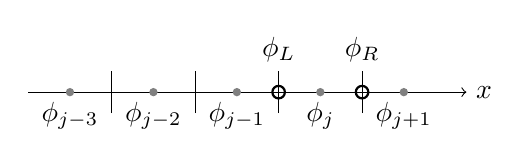
\begin{tikzpicture}[
  scale=0.53,
  cpnt/.style={fill=gray},
]

\draw [->] (-5,0) -- (5.5,0) node [right] {$x$};
\draw (-3,-0.5) -- (-3,0.5);
\draw (-1,-0.5) -- (-1,0.5);
\draw (1,-0.5) -- (1,0.5) node [above] {$\phi_L$};
\draw (3,-0.5) -- (3,0.5) node [above] {$\phi_R$};

\path [cpnt] (-4,0) circle [radius=0.1] node [below] {$\phi_{j-3}$};
\path [cpnt] (-2,0) circle [radius=0.1] node [below] {$\phi_{j-2}$};
\path [cpnt] (0,0) circle [radius=0.1] node [below] {$\phi_{j-1}$};
\path [cpnt] (2,0) circle [radius=0.1] node [below] {$\phi_j$};
\path [cpnt] (4,0) circle [radius=0.1] node [below] {$\phi_{j+1}$};
\draw [thick] (1,0) circle [radius=0.15];
\draw [thick] (3,0) circle [radius=0.15];

\end{tikzpicture}
\end{document}
}
	\caption{Schematics of one-dimensional linear transport discretisations with uniform wind and constant mesh spacing.  The von Neumann analysis starts with the 2-point approximation and subsequent analyses introduce additional points.  The 4-point approximation is constructed to mimic the configuration of typical stencils used by cubicFit, such as the stencil in figure~\ref{fig:stencil-interior}.  Cell centres are marked by grey filled circles and faces are marked by black open circles.  The uniform wind $u$ is from left to right.}
	\label{fig:vonNeumann}
\end{figure}


For stencils in some other distorted mesh regions, there is sufficient information to fit equation~\eqref{eqn:nine-poly}, but the resulting weights lead to an unstable transport scheme.  To detect these cases we evaluate the weights vector $\mathbf{w}$ against a set of constraints that are derived from a von Neumann stability analysis.

\subsection*{Von Neumann stability analysis}
The analysis starts by considering the linear transport equation that is continuous in time and discretised in space,
\begin{align}
	\frac{\partial \phi^{(n)}_j}{\partial t} &= -u \frac{\phi_R - \phi_L}{\Delta x}
\end{align}
with left- and right-hand face approximations, $\phi_L$ and $\phi_R$, separated by mesh spacing $\Delta x$ (figure~\ref{fig:vonNeumann-2}).  The face approximations are calculated as weighted sums of the neighbouring cell centre values,
\begin{align}
\phi_L &= w_u \phi_{j-1} + w_d \phi_j \\
\phi_R &= w_u \phi_j + w_d \phi_{j+1}
\end{align}
where we assume that the upwind weight $w_u$ and downwind weight $w_d$ are the same for both left- and right-hand faces.  We replace $\phi$ with the Fourier decomposition 
\begin{align}
	\phi_j^{(n)} &= A^n e^{\iu j k \Delta x}
\end{align}
where $\phi_j^{(n)}$ denotes the value of $\phi$ at position $j \Delta x$ and time level $(n)$, and $k$ is a wavenumber.  The wind $u$ is taken to be positive.  The amplification factor $A$ is constrained such that $|A| \leq 1$ and $\arg(A) < 0$ so that the solution has a physical phase speed and does not amplify.  Additionally, $A$ must be no less than the amplification factor for a first-order upwind scheme (in which $w_u = 1$, $w_d = 0$).  Similar analyses are performed for three-point approximations (figure~\ref{fig:vonNeumann-3}) and four-point approximations (figure~\ref{fig:vonNeumann-4}) to obtain the constraints on $\mathbf{w}$,
\begin{align}
	0.5 \leq w_u \leq 1 \\
	0 \leq w_d \leq 0.5 \\
	w_u - w_d \geq \max_{p\:\in\:P}(|w_p|)
\end{align}
where $P$ are the peripheral cells $\left\{ w_3, \ldots, w_n \right\}$.

The full-rank constraint and von Neumann stability constraints are used to select the most suitable subset of polynomial terms from equation~\eqref{eqn:nine-poly} (the subset includes the set itself).
The monitoring committee raised a concern about this procedure in our third meeting: which terms should be retained and which should be discarded?  Recent improvements address this issue.  We generate a set of candidate polynomials and select the candidate with the greatest number of terms that satisifies all constraints.  Candidate polynomials are generated such that high-order terms are discarded first.  More precisely, let
\begin{align}
	M(x, y) = { x^i y^j : i,j \geq 0 \text{ and } i+j \leq 3 }
\end{align}
be the set of all monomials of degree at most \num{3} in $x, y$.
A subset $S$ of $M(x,y)$ is ``dense'' if, whenever $x^a y^b$ and $x^c y^d$ are in $S$ with $a \leq c$ and $b \leq d$, then $x^i y^j$ is also in $S$ for all $a < i < c$, $b < j < d$.  The candidate polynomials are all the dense subsets of $M(x,y)$.  If multiple candidates with the same number of terms satisfy the constraints, the candidate with the best-conditioned matrix is chosen.

\subsection*{A new tracer transport test over steep terrain}

\begin{figure}
	\centering
	\subcaptionbox{Basic terrain-following mesh \label{fig:mesh-btf}}[.34\linewidth]{\includegraphics{../mountainAdvection-mesh-btf-1000/constant/mesh.pdf}}
	\subcaptionbox{Cut cell mesh \label{fig:mesh-cutCell}}[.34\linewidth]{\includegraphics{../mountainAdvection-mesh-cutCell-1000/constant/mesh.pdf}}
	\subcaptionbox{Slanted cell mesh \label{fig:mesh-slantedCell}}[.3\linewidth]{\includegraphics{../mountainAdvection-mesh-slantedCell-1000/constant/mesh.pdf}}
	\caption{The edges of the three meshes used in the two-dimensional tracer transport test.  The same wave-shaped mountain is represented by all three meshes.  The mesh spacing is $\Delta x = \SI{1000}{\meter}$ and $\Delta z = \SI{500}{\meter}$.  The peak mountain height is \SI{6}{\kilo\meter}.  Only part domain near the mountain is shown.  The entire domain is \SI{301}{\kilo\meter} wide and \SI{25}{\kilo\meter} high.}
	\label{fig:meshes}
\end{figure}

In MC3 we presented preliminary results of two-dimensional test case that used transported a stably-stratified thermal profile in a terrain-following wind field over orography.  We have since replaced this test with a variation of the standard orographic transport test by \citet{schaer2002}.  Test results are compared on a basic terrain-following (BTF) mesh (figure~\ref{fig:mesh-btf}), cut cell mesh (figure~\ref{fig:mesh-cutCell}), and slanted cell mesh (figure~\ref{fig:mesh-slantedCell}).  Three modifications were made to the standard test:
\begin{enumerate}
	\item The peak mountain height was raised to \SI{6}{\kilo\meter} in order to present a greater challenge to the cubicFit scheme.
	\item A terrain-following wind field was prescribed that is misaligned with all three meshes.  This was done to ensure that flow crosses mesh layers in all tests.
	\item The tracer was centred at the ground in order to assess transport accuracy over the lower boundary.
\end{enumerate}

\begin{figure}
	\centering
	\includegraphics{../fig-mountainAdvection-tracer/fig-mountainAdvection-tracer.pdf}
	\caption{Evolution of the tracer in the two-dimensional transport test over steep terrain.  The tracer is transported to the right over the wave-shaped terrain.  Tracer contours are every \SI{0.1}{\kilo\gram\per\meter\cubed}.  The result obtained using the cubicFit scheme on the basic terrain-following mesh is shown at $t=\SI{0}{\second}$, $t=\SI{5000}{\second}$ and $t=\SI{10000}{\second}$ with solid black contours. The analytic solution at $t=\SI{10000}{\second}$ is shown with dotted contours.
	The shaded box indicates the region that is plotted in figure~\ref{fig:mountainAdvection-errors}.
	\TODO{try to mask off below the mountain to hide the messy contouring}}
	\label{fig:mountainAdvection-tracer}
\end{figure}

Figure~\ref{fig:mountainAdvection-tracer} shows the evolution of the tracer with snapshots plotted at the initial time $t = \SI{0}{\second}$, half-way time $t = \SI{5000}{\second}$, and end time $t= \SI{10000}{\second}$.  At $t = \SI{5000}{\second}$ the tracer is positioned above the mountain and has been distorted by the terrain-following winds.  Once the tracer clears the mountain the analytic solution returns to its original shape (shown by dotted contours in figure~\ref{fig:mountainAdvection-tracer}).  The numerical result plotted with solid contours in figure~\ref{fig:mountainAdvection-tracer} was obtained on the basic terrain-following mesh using the cubicFit scheme.  Slight distortions are apparent at $t = \SI{10000}{\second}$ compared to the analytic solution.

\begin{figure}
	\centering
	\includegraphics{../fig-mountainAdvection-error/fig-mountainAdvection-error.pdf}
	\caption{Tracer contours at $t=\SI{10000}{\second}$ for the two-dimensional tracer transport tests.  A region in the lee of the mountain is plotted corresponding to the shaded area in figure~\ref{fig:mountainAdvection-tracer}.  Results are presented on BTF, cut cell and slanted cell meshes (shown in figure~\ref{fig:meshes}) using the linearUpwind and cubicFit transport schemes.  The numerical solutions are marked by solid black lines.  The analytic solution is marked by dotted lines.  Contours are every \SI{0.1}{\kilo\gram\per\meter\cubed}.  The error field is shaded in colour.}
	\label{fig:mountainAdvection-errors}
\end{figure}

To assess the accuracy of cubicFit, results are compared against a standard linearUpwind scheme \citepalias{openfoam}.  Numerical solutions are presented using solid contours in figure~\ref{fig:mountainAdvection-errors}.  The analytic solutions are shown with dotted contours and the error field is shaded in colour.
Errors are largest using the linearUpwind scheme on the cut cell mesh.  Results are improved using the linearUpwind scheme with slanted cell mesh or basic terrain-following mesh.  A great improvement is found using the cubicFit scheme, which is seen to be largely insensitive to the choice of mesh.

We expect that few or no further modifications to the transport scheme will be needed.   Since our meeting in May 2016, we realised that further experiments were needed to demonstrate that the cubicFit scheme is suitable for non-quadrilateral meshes.  To address this, we have performed tests on a sphere using standard deformational flow tests by \citet{lauritzen2012} on hexagonal icosahedra.
Work is now underway to document the cubicFit scheme and experimental results.
We intend to submit a manuscript to the Journal of Computational Physics in early 2017.

\section{Future research}
\label{sec:future}

Work has progressed well since the previous meeting in May 2016, though an additional 1--2 months was taken with additional transport tests on the sphere.  Here we present a revised timeline of tasks:
\begin{description}
\item[January 2017]{Submit a manuscript documenting the cubicFit transport scheme to the Journal of Computational Physics.}
\item[February 2017]{Begin work on generalising the Charney--Phillips staggering for arbitrary meshes.  Start by verifying that existing test cases, such as those from \citet{arakawa-konor1996}, are able to excite the Lorenz computational mode using the nonhydrostatic model by \citet{weller-shahrokhi2014}.}
\item[April 2017]{Complete modifications to the nonhydrostatic model to enable execution using the generalised Charney--Phillips staggering.  The model should include a simple transport scheme for potential temperature.  The model will have a fully-explicit formulation.}
\item[Summer 2017]{Time permitting, the model should be improved using a more accurate transport scheme.  Such a scheme will likely be based on the cubicFit scheme that we have already implemented.  The model might also be extended with a semi-implicit treatment of gravity waves.}
\item[Autumn 2017]{Complete main thesis chapters (outlined in section~\ref{sec:thesis-plan}) including all test results.}
\item[Early 2018]{Complete PhD.}
\end{description}

\section{Thesis plan}
\label{sec:thesis-plan}

What follows is an outline of the main chapters of my thesis.

\titlespacing\subsubsection{0pt}{0.8em plus 4pt minus 2pt}{0.4em plus 2pt minus 2pt}

\subsubsection*{A new mesh for representing terrain}
\begin{itemize}
	\setlength\itemsep{0.1em}
	\item Introduce existing types of mesh
	\item Describe the new slanted cell method
\end{itemize}

\subsubsection*{A new transport scheme for steep slopes}
\begin{itemize}
	\setlength\itemsep{0.1em}
	\item Document the cubicFit transport scheme
	\item Two-dimensional transport tests over steep slopes
	\item Deformational transport tests on a spherical Earth
\end{itemize}
	
\subsubsection*{A generalisation of the Charney--Phillips staggering}
\begin{itemize}
	\setlength\itemsep{0.1em}
	\item Describe the generalised Charney--Phillips formulation
	\item A nonhydrostatic model for arbitrary meshes
	\item A test of a quiescent atmosphere above steep slopes
	\item One or two tests that excite the Lorenz computational mode
	\item Mountain waves test case
\end{itemize}

\section{Personal development}
This section highlights some of my recent personal developments.  A complete training record is available in the appendix.

I hope to attend two conferences next year.  Hilary recommended PDEs on the Sphere as an excellent venue to present my work to an audience of numerical geoscientists.  I would also like to attend SciCADE, a conference on Scientific Computation and Differential Equations, in order to meet numerical scientists and mathematicians working in other disciplines.

I have gained more experience as a reviewer, having provided feedback on the MSc dissertation of Hilary's most recent MSc student, Christiana Skea.  We were extremely pleased that Christiana was awarded the MSc dissertation prize for her work.  I have also reviewed a second manuscript for Monthly Weather Review.

\bibliographystyle{ametsoc2014}                                                 
\bibliography{references}

\newpage

\section*{Appendix}

\titlespacing\subsection{0pt}{0.8em plus 4pt minus 2pt}{0.2em plus 2pt minus 2pt}

\subsection*{Mathematics modules}
\footnotesize
\begin{tabular}{l l l l}
Spring 2016	& MA3NAT & Numerical Analysis II & unassessed \\
Spring 2015	& MAMNSP & Numerical Solution of Partial Differential Equations  & 78\% \\
\end{tabular}

\subsection*{RRDP modules}
\begin{tabular}{l l}
Summer 2017	& Organising conferences \\
28 Feb 2017	& Getting your first post-doc position \\
9 Nov 2016      & Open Access and research data management \\
24 Mar 2016	& Voice coaching: looking after your voice \\
26--27 Jan 2016 & Preparing to teach (introduction, marking \& feedback, leading small groups) \\
2 Dec 2015	& An essential guide to critical academic writing \\
17 Nov 2015	& Understanding the UK higher education context \\
19 May 2015	& How to avoid plagiarism \\
10 Mar 2015	& How to write a literature review \\
19 Feb 2015	& How to write a paper \\
\end{tabular}

\subsection*{External courses}
\begin{tabular}{l l}
June 2016 & Dynamical core intercomparison project summer school, NCAR \\
13 May 2016 & Peer review: the nuts and bolts, Sense about Science \\
June 2015 & Advanced numerical methods for Earth-system modelling, ECMWF \\
\end{tabular}

\subsection*{Conferences and workshops}
\begin{tabularx}{\linewidth}{l l X}
September 2017 & & \href{https://sites.google.com/site/scicade2017/}{SciCADE}, University of Bath \\
April 2017 & & \href{https://forge.ipsl.jussieu.fr/heat/wiki/PDEs2017}{PDEs on the Sphere}, Paris \\
February 2017 & Speaker & Numerical Methods for Geophysical Fluid Dynamics, Imperial College London \\
October 2016 & Speaker & \href{http://www.ecmwf.int/en/learning/workshops-and-seminars/workshop-numerical-and-computational-methods-simulation-all-scale-geophysical-flows}{Numerical and computational methods for simulation of all-scale geophysical flows}, ECMWF \\
July 2016 & Attendee & 1st GungHo Network meeting, Daresbury Laboratory \\
November 2015 & Attendee & GungHo workshop on next generation weather and climate prediction, UK Met Office \\
June 2015 & Attendee & Hoskins@70 \\
June 2015 & Poster & SCENARIO DTP conference \\
March 2015 & Speaker & \href{http://www.icms.org.uk/workshop.php?id=334}{Galerkin methods with applications in weather and climate forecasting}, ICMS \\
\end{tabularx}

\subsection*{Teaching}
\begin{tabular}{l l l}
Oct 2016 & Teaching assistant & MTMW11 fluid dynamics \\
Oct 2015 & Teaching assistant & MTMG02 atmospheric physics \\
Sep 2015 & Teaching assistant & NCAS summer school \\
Sep 2014 & Course teacher & MPE python and linux short course \\
\end{tabular}

\subsection*{Visits and collaborations}
\begin{tabularx}{\linewidth}{l X}
July 2016 & Organised visit from \href{https://www.youtube.com/user/SimonOxfPhys}{Simon Clark}, stratospheric PhD researcher and YouTube vlogger \\
Summer 2016 & Worked with Hilary's MSc student, Christiana Skea, studying variable timestepping for ODEs \\
June 2016 & Visited NCAR, hosted by Ram Nair \\
2015 -- 2016 & Coauthoring an article about dimensionally-split and multidimensional advection schemes, written with Hilary, her former student Yumeng Chen, and Stephen Pring at the UK Met Office \\
\end{tabularx}


\subsection*{Outreach}
\begin{tabular}{l l l}
14 Jul 2015 & Schools physicist of the year awards \\
14 Jun 2015 & East Reading festival \\
15 Feb 2015 & Brighton science festival \\
\end{tabular}

\subsection*{Presentations}
\begin{tabularx}{\linewidth}{l l X}
17 Nov 2016 & Comp. Atmos. Dyn. group & \\
9 Nov 2016 & PhD group & \\
31 Oct 2016 & HHH group & \\
22 Sep 2016 & PhD poster session & Improving numerical accuracy over steep slopes \\
23 Mar 2016 & Quo Vadis & Numerical representation of orography in dynamical cores (honourable mention) \\
17 Feb 2016 & PhD group & Multidimensional advection schemes for arbitrary meshes \\
9 Feb 2016 & Mesoscale group & Curl-free pressure gradients for accurate modelling of cold air pools \\
19 Oct 2015 & HHH group & Improving modelled mountain flows with alternative representations of terrain \\
27 Apr 2015 & HHH group & A like-for-like comparison between terrain following and cut cell grids \\
21 Apr 2015 & PhD group & Discrete vector calculus on Arakawa C grids \\
12 Feb 2015 & UK Met Office & Poster presentation for Met Office Academic Partnership \\
18 Jan 2015 & PhD group & Python and linux tips \\
17 Dec 2014 & MPECDT jamboree & Poster presentation for Mathematics for Planet Earth Centre for Doctoral Training jamboree \\
12 Sep 2014 & Lunchtime seminar  & Gain control of your documents and code: hands-on with revision control and build automation \\
\end{tabularx}

\end{document}
